\documentclass[11pt]{article}
\usepackage[hmargin=1in,vmargin=1in]{geometry}
\usepackage{xcolor}
\usepackage{amsmath}
\usepackage{graphicx} % Required for inserting images
\usepackage{amsmath,amssymb,amsfonts,url,sectsty,framed,tcolorbox,framed}
\usepackage{nicematrix}
\usepackage{amssymb}
\usepackage{algorithm2e}
\setcounter{MaxMatrixCols}{16}
\usepackage{tikz}
\usepackage{hyperref}
\usetikzlibrary{decorations.pathreplacing}
\newcommand{\pf}{{\bf Proof: }}
\newtheorem{theorem}{Theorem}
\newtheorem{lemma}{Lemma}
\newtheorem{proposition}{Proposition}
\newtheorem{definition}{Definition}
\newtheorem{remark}{Remark}
\newcommand{\zbar}{\raisebox{0.2ex}{--}\kern-0.6em Z}
\newcommand{\qed}{\hfill \rule{2mm}{2mm}}
\usepackage{titlesec}

\setcounter{secnumdepth}{4}
\titleclass{\subsubsubsection}{straight}[\subsection]
\newcounter{subsubsubsection}[subsubsection]
\renewcommand{\thesubsubsubsection}{\thesubsubsection.\arabic{subsubsubsection}}
\titleformat{\subsubsubsection}{\normalfont\normalsize\bfseries}{\thesubsubsubsection}{1em}{}
\titlespacing*{\subsubsubsection}{0pt}{3.25ex plus 1ex minus .2ex}{1.5ex plus .2ex}

\setcounter{tocdepth}{4}

\begin{document}



%%%%%%%%%%%%%%%%%%%%%%%%%%%%%%%%%%%%%%%%%%%%%%%%%%%%%%%%%%%%%%%%%%%%%
\noindent
\rule{\textwidth}{1pt}
\begin{center}
{\bf [CS304] Introduction to Cryptography and Network Security}
\end{center}
Course Instructor: Dr. Dibyendu Roy \hfill Winter 2022-2023\\
Scribed by: Chitranshi Srivastava (202051055) \hfill Lecture 23 and 24 (Week 13)
\\
\rule{\textwidth}{1pt}
%%%%%%%%%%%%%%%%%%%%%%%%%%%%%%%%%%%%%%%%%%%%%%%%%%%%%%%%%%%
%write here
\section{Secured Sockets Layer}
Most of the cryptographic protocols are based on three cryptographic primitives:
\begin{itemize}
    \item Symmetric Key Encryption Algorithms. These are preferred as computations in Public Key Cryptography are usually harder than symmetric key cryptography.
    \item Key Exchange Protocol so as to get the common shared key at both ends. A signature mechanism to verify the authenticity of the source and the public keys to avoid attacks such as Man in the Middle Attack.
    \item Message Authentication Code for authenticating the encrypted data. It will give the assurance that you have received the message from the correct party and the message has not been altered.
\end{itemize}
SSL protocol is implemented everywhere in HTTPS. It provides a secure communication between two parties where you're going to perform a key-exchange, encryption using symmetric key, a signature or authenticating the public keys, perform a Message Authentication Code to authenticate the message. \\
\newline
It starts with a connection. A \textbf{connection} is a transport that provides a suitable type of service. The connections are transient. Every connection is associated with one session. A \textbf{session} is when you hit a HTTPS website, you establish a session with their server. The session will going to have a time period and during this period you will be exchanging the data. All this data exchange will be completely encrypted. Sessions
are created by the Handshake Protocol. Sessions define a set of cryptographic security parameters, which can be shared among multiple connections. Sessions are used to avoid the expensive negotiation of new security parameters for each connection.\\
\newline
A session state is defined by the following parameters:
\begin{enumerate}
    \item \textbf{Session identifier:} An arbitrary byte sequence chosen by the server to identify an active or resumable session state. 
    \item \textbf{Peer certificate:} An X509.v3 certificate of the peer. This element of the state may be null. It is usually a signed public key. If we say that you are buying a SSL certificate that means you are basically getting your public key signed by a certified authority (using their secret key so that it is verifiable by everyone that the authority has authorised it). This certificate is used by the receiver to verify your public key. One such certified authority is X509.v3.
    \item \textbf{Compression method:} The algorithm used to compress data prior to encryption. Corresponding to this algorithm, there is a decompression algorithm.
    \item \textbf{Cipher spec:} It specifies the bulk data encryption algorithm (such as null, AES, etc.), a hash algorithm (such as MD5 or SHA-1) used for MAC calculation, a mechanism for key exchange (Diffie-Hellman, ECDH). It also defines cryptographic attributes such as the hash size.
    \item \textbf{Master secret:} 48-byte secret shared between the client and server. It is used to generate certain keys such as key for encrypting the data and a key for generating MAC.
    \item \textbf{Is resumable:} A flag indicating whether the session can be used to initiate new connections.
\end{enumerate}

A connection state is defined by the following parameters:
\begin{enumerate}
    \item \textbf{Server and client random:} Byte sequences that are chosen by the server and client for each connection. These are generated individually at the client and the server side. These numbers are involved in certain computation to prevent certain attacks.
    \item \textbf{Server write MAC secret:} The secret key used in MAC operations on data sent by the server. It is same at the client and the server side.
    \item \textbf{Client write MAC secret:} The symmetric key used in MAC operations on data sent by the client.
    \item \textbf{Server write key:} The symmetric encryption key for data encrypted by the server and decrypted by the client.
    \item \textbf{Client write key:} The symmetric encryption key for data encrypted by the client and decrypted by the server.
    \item \textbf{Initialization vectors:} When a block cipher in CBC mode is used, an initialization vector (IV) is maintained for each key. This field is first initialized by the SSL Handshake Protocol. Thereafter, the final ciphertext block from each record is preserved for use as the IV with the following record.
    \item \textbf{Sequence numbers:} Each party maintains separate sequence numbers for transmitted and received messages for each connection. When a party sends or receives a “change cipher spec message”, the appropriate sequence number is set to zero. Sequence numbers may not exceed $2^{64} - 1$.
\end{enumerate}

\subsection{SSL Record Protocol}
There are certain protocols involved in the entire SSL. The first protocol involved is the SSL Record Protocol. This protocol provides two services for SSL connections:
\begin{enumerate}
    \item \textbf{Confidentiality:} The Handshake Protocol defines a shared secret key that is used for conventional encryption of SSL payloads.
    \item \textbf{Message Integrity:} The Handshake Protocol also defines a shared secret key that is used to form a message authentication code (MAC).
\end{enumerate}
Given a data, let's say you have a packet, first break the packet into multiple blocks of fixed size. The length of the block depends on the protocol version. On each block, perform the compression algorithm. It will compress the fragmented data to a fixed length size. On this compressed data, the MAC will be generated using the MAC Secret Key. This MAC will be concatenated with the compresses data. Now this data, that is, compressed data concatenated with MAC will be encrypted using an encryption algorithm. After encryption, a header will be added before the encrypted data. The header contain contains public information that we do not want to encrypt. This will be the complete packet that will be transferred either from client to server or vice-versa. A flowchart for the above described process is given below.

\begin{center}
    \tikzset{every picture/.style={line width=0.75pt}} %set default line width to 0.75pt        
    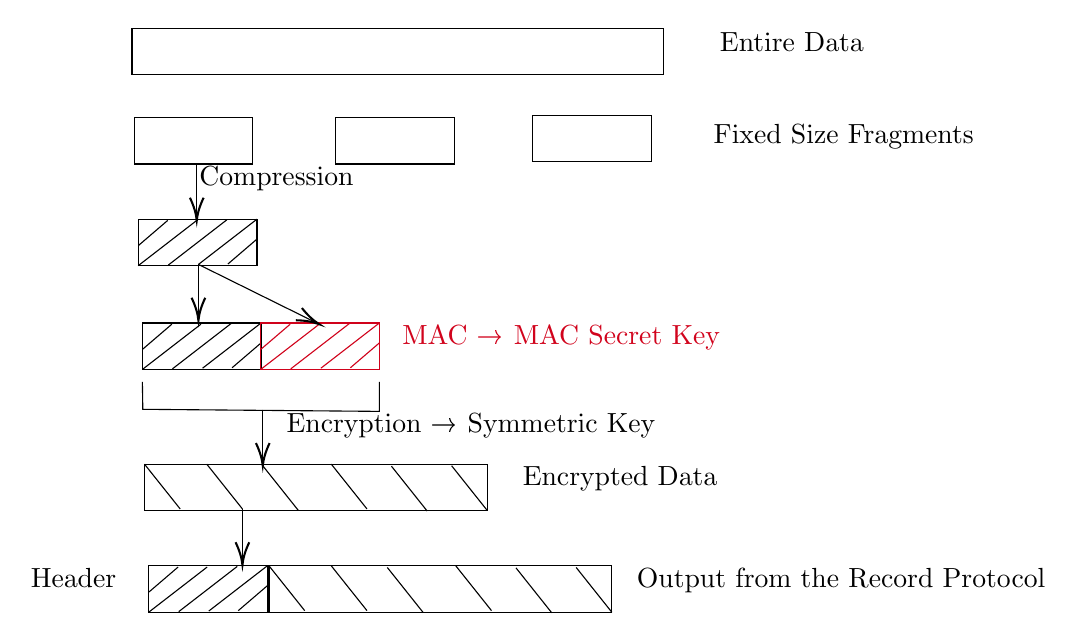
\begin{tikzpicture}[x=0.75pt,y=0.75pt,yscale=-1,xscale=1]
        \draw   (98,58) -- (354.2,58) -- (354.2,80.4) -- (98,80.4) -- cycle ;
        \draw   (99,101) -- (156.2,101) -- (156.2,123.4) -- (99,123.4) -- cycle ;
        \draw   (196,101) -- (253.2,101) -- (253.2,123.4) -- (196,123.4) -- cycle ;
        \draw   (291,100) -- (348.2,100) -- (348.2,122.4) -- (291,122.4) -- cycle ;
        \draw    (129.2,123.6) -- (129.2,148.6) ;
        \draw [shift={(129.2,150.6)}, rotate = 270] [color={rgb, 255:red, 0; green, 0; blue, 0 }  ][line width=0.75]    (10.93,-3.29) .. controls (6.95,-1.4) and (3.31,-0.3) .. (0,0) .. controls (3.31,0.3) and (6.95,1.4) .. (10.93,3.29)   ;
        \draw   (101,150) -- (158.2,150) -- (158.2,172.4) -- (101,172.4) -- cycle ;
        \draw    (101.2,162.6) -- (115.2,150.6) ;
        \draw    (101,172.4) -- (129.2,150.6) ;
        \draw    (115.5,172.1) -- (143.7,150.3) ; 
        \draw    (130,171.8) -- (158.2,150) ;
        \draw    (144.2,171.6) -- (158.2,159.6) ;
        \draw   (103,200) -- (160.2,200) -- (160.2,222.4) -- (103,222.4) -- cycle ;
        \draw    (103.2,212.6) -- (117.2,200.6) ;
        \draw    (103,222.4) -- (131.2,200.6) ;
        \draw    (117.5,222.1) -- (145.7,200.3) ; 
        \draw    (132,221.8) -- (160.2,200) ;
        \draw    (146.2,221.6) -- (160.2,209.6) ; 
        \draw  [color={rgb, 255:red, 208; green, 2; blue, 27 }  ,draw opacity=1 ] (160,200) -- (217.2,200) -- (217.2,222.4) -- (160,222.4) -- cycle ;
        \draw [color={rgb, 255:red, 208; green, 2; blue, 27 }  ,draw opacity=1 ]   (160.2,212.6) -- (174.2,200.6) ;
        \draw [color={rgb, 255:red, 208; green, 2; blue, 27 }  ,draw opacity=1 ]   (160,222.4) -- (188.2,200.6) ; 
        \draw [color={rgb, 255:red, 208; green, 2; blue, 27 }  ,draw opacity=1 ]   (174.5,222.1) -- (202.7,200.3) ;
        \draw [color={rgb, 255:red, 208; green, 2; blue, 27 }  ,draw opacity=1 ]   (189,221.8) -- (217.2,200) ;
        \draw [color={rgb, 255:red, 208; green, 2; blue, 27 }  ,draw opacity=1 ]   (203.2,221.6) -- (217.2,209.6) ;
        \draw    (130,171.8) -- (130,196.8) ;
        \draw [shift={(130,198.8)}, rotate = 270] [color={rgb, 255:red, 0; green, 0; blue, 0 }  ][line width=0.75]    (10.93,-3.29) .. controls (6.95,-1.4) and (3.31,-0.3) .. (0,0) .. controls (3.31,0.3) and (6.95,1.4) .. (10.93,3.29)   ;
        \draw    (130,171.8) -- (186.41,199.71) ;
        \draw [shift={(188.2,200.6)}, rotate = 206.33] [color={rgb, 255:red, 0; green, 0; blue, 0 }  ][line width=0.75]    (10.93,-3.29) .. controls (6.95,-1.4) and (3.31,-0.3) .. (0,0) .. controls (3.31,0.3) and (6.95,1.4) .. (10.93,3.29)   ;
        \draw    (103,228.4) -- (103.2,241.6) -- (171.19,242.2) -- (217.2,242.6) -- (217.2,228.4) ;
        \draw    (161,241.8) -- (161,266.8) ;
        \draw [shift={(161,268.8)}, rotate = 270] [color={rgb, 255:red, 0; green, 0; blue, 0 }  ][line width=0.75]    (10.93,-3.29) .. controls (6.95,-1.4) and (3.31,-0.3) .. (0,0) .. controls (3.31,0.3) and (6.95,1.4) .. (10.93,3.29)   ;
        \draw   (104,268) -- (269.2,268) -- (269.2,290.4) -- (104,290.4) -- cycle ;
        \draw    (104,268) -- (121.2,289.6) ;
        \draw    (134,268) -- (151.2,289.6) ;
        \draw    (161,268.8) -- (178.2,290.4) ;
        \draw    (194,268) -- (211.2,289.6) ;
        \draw    (223,269) -- (240.2,290.6) ;
        \draw    (252,268.8) -- (269.2,290.4) ;
        \draw   (164,317) -- (329.2,317) -- (329.2,339.4) -- (164,339.4) -- cycle ;
        \draw    (164,317) -- (181.2,338.6) ;
        \draw    (194,317) -- (211.2,338.6) ;
        \draw    (221,317.8) -- (238.2,339.4) ;
        \draw    (254,317) -- (271.2,338.6) ;
        \draw    (283,318) -- (300.2,339.6) ;
        \draw    (312,317.8) -- (329.2,339.4) ;
        \draw   (106,317) -- (163.2,317) -- (163.2,339.4) -- (106,339.4) -- cycle ;
        \draw    (106.2,329.6) -- (120.2,317.6) ; 
        \draw    (106,339.4) -- (134.2,317.6) ;
        \draw    (120.5,339.1) -- (148.7,317.3) ;
        \draw    (135,338.8) -- (163.2,317) ;
        \draw    (149.2,338.6) -- (163.2,326.6) ;
        \draw    (151.2,289.6) -- (151.2,314.6) ;
        \draw [shift={(151.2,316.6)}, rotate = 270] [color={rgb, 255:red, 0; green, 0; blue, 0 }  ][line width=0.75]    (10.93,-3.29) .. controls (6.95,-1.4) and (3.31,-0.3) .. (0,0) .. controls (3.31,0.3) and (6.95,1.4) .. (10.93,3.29)   ;

        \draw (380,59) node [anchor=north west][inner sep=0.75pt]   [align=left] {Entire Data};  
        \draw (377,103) node [anchor=north west][inner sep=0.75pt]   [align=left] {Fixed Size Fragments};
        \draw (129.2,123.6) node [anchor=north west][inner sep=0.75pt]   [align=left] {Compression};
        \draw (227,200) node [anchor=north west][inner sep=0.75pt]   [align=left] {\textcolor[rgb]{0.82,0.01,0.11}{MAC → MAC Secret Key}};
        \draw (171.19,242.2) node [anchor=north west][inner sep=0.75pt]   [align=left] {Encryption → Symmetric Key};
        \draw (285,268) node [anchor=north west][inner sep=0.75pt]   [align=left] {Encrypted Data};
        \draw (48,317) node [anchor=north west][inner sep=0.75pt]   [align=left] {Header};
        \draw (340,317) node [anchor=north west][inner sep=0.75pt]   [align=left] {Output from the Record Protocol};
    \end{tikzpicture}
\end{center}
Now, suppose we have received this data from the server. The length of the header part is known, hence, it is discarded from the packet and any necessary information required is taken from it. Now, we will first perform the decryption and we will get the compressed data concatenated with the MAC. The length of MAC is known and hence that part will be taken away. Therefore, we have the compressed data from which we will generate a the MAC. If the generated MAC matches with the received MAC, then the data is authenticated. If it is matching, we will perform the decompression operation to get the original data contained in the packet.\\
\newline
The two keys required are MAC Secret Key and the key used for encryption. These two keys will be same at client and server side. The MAC that is generated is computed as:\\
MAC: hash(MAC\_write\_secret $||$  pad2  $||$ hash(MAC\_write\_secret $||$  pad1 $||$ seq\_num $||$ SSLCompressed.type $||$ SSLCompressed.length $||$ SSLCompressed.fragment))\\
\newline
The list of encryption algorithms supported by SSL is given below.
\begin{center}
    AES, IDEA, RC2-40, DES-40, DES, 3DES, Fortezza, RC4-40, RC4-128
\end{center}
There will be a negotiation between the client and the server and they will agree on one encryption algorithm.\\
\newline
Header is basically some public information that is not required to be encrypted. The header contain the following information.
\begin{itemize}
    \item Content Type (8 bits): The type of data
    \item Major Version (8 bits): Suppose you are using version 3 of SSL, then major version will be 3.
    \item Minor Version (8 bits): Suppose you are using version 3 of SSL, then minor version will be 0.
    \item Compressed Length (16 bits): length of the compressed data.
\end{itemize}

\subsection{Change Cipher Spec Protocol}
 Another protocol used in SSL is Change Cipher Spec Protocol. It basically update the cipher suite to be used on this connection. Suppose you are using the RC4 for encrypting the data. After certain time, the client and server want to change the encryption mechanism and want to use AES. This protocol is used in such scenarios.

 \subsection{Alert Protocol}
 Its main function is to give some kind of alert if something is wrong. A list of few(not all) alerts is given below alongwith the description when these alerts are given by the Alert Protocol.
 \begin{itemize}
     \item  \textbf{unexpected\_message:} An inappropriate message was received.
     \item \textbf{bad\_record\_mac:} An incorrect MAC was received.
     \item \textbf{decompression\_failure:} The decompression function received improper input (e.g., unable to decompress or decompress to greater than maximum allowable length).
     \item \textbf{handshake\_failure:} Sender was unable to negotiate an acceptable set of security parameters given the options available.
     \item \textbf{illegal\_parameter:} A field in a handshake message was out of range or inconsistent with other fields.
     \item \textbf{close\_notify:} Notifies the recipient that the sender will not send any more messages on this connection. Each party is required to send a close\_notify alert before closing the write side of a connection.
    \item \textbf{bad\_certificate:} A received certificate was corrupt (e.g., contained a signature that did not verify).
    \item \textbf{unsupported\_certificate:} The type of the received certificate is not supported.
    \item \textbf{certificate\_revoked:} A certificate has been revoked by its signer.
    \item \textbf{certificate\_expired:} A certificate has expired.
    \item \textbf{certificate\_unknown:} Some other unspecified issue arose in processing the certificate, rendering it unacceptable.
 \end{itemize}
 
 \subsection{Handshake Protocol}
It is the most important protocol of the SSL. It performs the handshaking between the two parties and generate a common secret key. Using this secret key, the encryption and MAC keys are generated which are used for encryption and MAC generation.

\begin{figure}[htbp]
   \centering
   \includegraphics[width=0.5\textwidth]{handshake.JPG}
   \caption{Action of Handshake Protocol}   
\end{figure}

Let us understand the working of the protocol. The initiation of communication between client and server will be done by the client. The first message from the client side is named as a hello message (client\_hello). Some data will be passed from client to server in this hello message. In reply, the server will send its hello message (server\_hello). It contains some data which will be used for further communication. Then the server, will send the certificate (signed public key) to the client and will begin the key exchange. It will send some data which will be required for key exchange(server\_key\_exchange). Server might ask the client for the certificate for client's browser (certificate\_request). Finally, the server will send the hello done message. Using this, it can be identified that the server's hello is done here.\\
\newline
In reply, the client will send the certificate if requested. Then client will send the key-exchange data (client\_key\_exchange). If the client and server are agreeing on Diffie-Hellman key exchange, then they will have to share their Diffie-Hellman Public Keys with each other, otherwise key cannot be established. The client will verify the certificate given by the server and send a reply (certificate\_verify). The will send a cipher spec message (change\_cipher\_spec) indicating what are the ciphers client supports. Afterwards, the client will send a finish message (finished). The server will reply with a cipher spec message (change\_cipher\_spec) indicating if the server can support the requested cipher or not or some algorithm for further communication. If it is supported, then the server will send a finish message (finished).\\
\newline
Now, let us see what are the information which will be a part of the different messages from the client side and the server side.
\begin{enumerate}
    \item \textbf{client\_hello\_message:} It contains the following data:
    \begin{itemize}
        \item Version: the version of SSL protocol that client supports
        \item Random: A client-generated random structure consisting of a 32-bit timestamp and 28 bytes generated by a secure random number generator.
        \item \textbf{Session ID:} A variable-length session identifier. A nonzero value indicates that the client wishes to update the parameters of an existing connection or to create a new connection on this session. A zero value indicates that the client wishes to establish a new connection on a new session.
        \item \textbf{Cipher Suite:} This is a list that contains the combinations of cryptographic algorithms supported by the client, in decreasing order of preference. Each element of the list (each cipher suite) defines both a key exchange algorithm and a CipherSpec; these are discussed subsequently.
        \item \textbf{Compression Method:} This is a list of the compression methods the client supports.
    \end{itemize}
    After sending the client\_hello\_message, the client waits for the server\_hello\_message, which contains the same parameters as the client\_hello\_message. Let us now go through the contents of the Cipher Suite parameter in the hello messages.\\
    \newline
    The first element of the Ciphersuite parameter is the key exchange method. The following key exchange methods are supported:
    
    \begin{itemize}
        \item \textbf{RSA:} The secret key is encrypted with the receiver’s RSA public key. A publickey certificate for the receiver’s key must be made available.
        \item \textbf{Fixed Diffie-Hellman:} This is a Diffie–Hellman key exchange in which the server’s certificate contains the Diffie–Hellman public parameters signed by the certificate authority (CA). That is, the public-key certificate contains the Diffie–Hellman public-key parameters. The client provides its Diffie–Hellman public-key parameters either in a certificate, if client authentication is required, or in a key exchange message. This method results in a fixed secret key between two peers based on the Diffie–Hellman calculation using the fixed public keys.
        \item \textbf{Ephemeral Diffie-Hellman:} This technique is used to create ephemeral (temporary, one-time) secret keys. In this case, the Diffie–Hellman public keys are exchanged and signed using the sender’s private RSA or DSS key. The receiver can use the corresponding public key to verify the signature. Certificates are used to authenticate the public keys.
        \item \textbf{Anonymous Diffie-Hellman:} The base Diffie–Hellman algorithm is used with no authentication. That is, each side sends its public Diffie–Hellman parameters to the other with no authentication. This approach is vulnerable to man-in-the-middle attacks.
    \end{itemize}
    Following the definition of a key exchange method is the CipherSpec, which includes the following fields:
    \begin{itemize}
        \item \textbf{CipherAlgorithm:} Any of the algorithms mentioned earlier: RC4, RC2, DES, 3DES, DES40, or IDEA
        \item \textbf{MACAlgorithm:} MD5 or SHA-1
        \item \textbf{CipherType:} Stream or Block
        \item \textbf{IsExportable:} True or False
        \item \textbf{HashSize:} 0, 16 (for MD5), or 20 (for SHA-1) bytes
        \item \textbf{Key Material:} A sequence of bytes that contain data used in generating the write keys
        \item \textbf{IV Size:} The size of the Initialization Value for Cipher Block Chaining (CBC) encryption
    \end{itemize}

    \item \textbf{server\_key\_exchange message:} It is not required in two instances: (1) The server has sent a certificate with fixed Diffie–Hellman parameters; or (2) RSA key exchange is to be used. The server\_key\_exchange message is needed for the following:
    \begin{itemize}
        \item \textbf{Anonymous Diffie–Hellman:} The message content consists of the two global Diffie–Hellman values (a prime number and a primitive root of that number) plus the server’s public Diffie–Hellman key.
        \item \textbf{Ephemeral Diffie–Hellman:} The message content includes the three Diffie–Hellman parameters provided for anonymous Diffie–Hellman plus a signature of those parameters.
        \item \textbf{RSA key exchange (in which the server is using RSA but has a signature-only RSA key):} Accordingly, the client cannot simply send a secret key encrypted with the server’s public key. Instead, the server must create a temporary RSA public/private key pair and use the server\_key\_exchange message to send the public key. The message content includes the two parameters of the temporary RSA public key plus a signature of those parameters.
    \end{itemize}
    As usual, a signature is created by taking the hash of a message and encrypting it with the sender’s private key. In this case, the hash is defined as:
    \begin{center}
        hash(ClientHello.random $||$ ServerHello.random $||$ ServerParams)
    \end{center}
    So the hash covers not only the Diffie–Hellman or RSA parameters but also the two nonces from the initial hello messages.

    \item \textbf{client\_key\_exchange message:} The content of the message depends on the type of key exchange, as follows:
    \begin{itemize}
        \item \textbf{RSA:} The client generates a 48-byte pre-master secret and encrypts with the public key from the server’s certificate or temporary RSA key from a server\_key\_exchange message. Its use to compute a master secret is explained later.
        \item \textbf{Ephemeral or Anonymous Diffie–Hellman:} The client’s public Diffie–Hellman parameters are sent.
        \item \textbf{Fixed Diffie–Hellman:} The client’s public Diffie–Hellman parameters were sent in a certificate message, so the content of this message is null.
    \end{itemize}

    \item \textbf{certificate\_verify message:} Client may send a certificate\_verify message where the client is going to generate two hash values.
    \begin{itemize}
        \item CertificateVerify.signature.md5\_hash = MD5(master\_secret $||$ pad\_2 $||$ MD5(handshake\_messages $||$ master\_secret $||$ pad\_1));
        \item CertificateVerify.signature.sha\_hash = SHA(master\_secret $||$ pad\_2 $||$ SHA(handshake\_messages $||$ master\_secret $||$ pad\_1));
    \end{itemize}
    The master\_secret is generated using the pre-master secret key. On this hash value the client will produce a signature. This entire hash will be signed using the private key of the client and will be sent to the server, if the client wants the certificate\_verify message.

    \item \textbf{change\_cipher\_spec message:} The client sends a change\_cipher\_spec message and copies the pending CipherSpec into the current CipherSpec. The client then immediately sends the finished message. The contents of the finished message are concatenation of two hash values. These hash values are given below:
    \begin{itemize}
        \item MD5(master\_secret $||$ pad\_2 $||$ MD5(handshake\_messages $||$ Sender $||$ master\_secret $||$ pad\_1));
        \item SHA(master\_secret $||$ pad\_2 $||$ SHA(handshake\_messages $||$ Sender $||$ master\_secret $||$ pad\_1));
    \end{itemize}

    \item  In response to the above mentioned two messages, the server sends its own change\_cippher\_spec message and transfers the pending to the current CipherSpec, and sends its finished message.
\end{enumerate}

Let us now see how the master secret key is generated using the pre-master key. The master secret key is generated as:\\
master\_secret = MD5(pre\_master\_secret $||$ SHA(A $||$ pre\_master\_secret $||$ ClientHello.random $||$ ServerHello.random)) $||$ MD5(pre\_master\_secret $||$ SHA(BB $||$ pre\_master\_secret $||$ ClientHello.random $||$ ServerHello.random)) $||$ MD5(pre\_master\_secret $||$ SHA(CCC $||$ pre\_master\_secret $||$ ClientHello.random $||$ ServerHello.random))\\
A, BB and CCC are pre-defined constants. Now, both the parties have master secret key. The involvement of random numbers in master secret key is explained below.\\
\newline
Suppose, they are having only fixed Diffie-Hellman (no ephemeral Diffie-Hellman). If we have the Diffie-Hellman public keys and we perform Diffie Hellman Key Exchange for multiple times, you will lead to have the same secret key everytime. Now, let us say one session has been corrupted and some data has been leaked (not the secret key). But you can see that the master secret will be used for encryption and the MAC generation. If one session is corrupted, then the second session cannot be corrupted because we are involving a random number as an input to a hash function which are different for every session. Hence, the master secret key is different for every session. These values serve as nonces and are used during key exchange to prevent replay attacks.\\
\newline
Using the master secret key, we will be generating a block of keys. This key generation will be continue till you have sufficient amount of keys. \\
key\_block = MD5(master\_secret $||$ SHA(A $||$ master\_secret $||$ ServerHello.random $||$ ClientHello.random)) $||$ MD5(master\_secret $||$ SHA(BB $||$ master\_secret $||$ ServerHello.random $||$ ClientHello.random)) $||$ MD5(master\_secret $||$ SHA(CCC $||$ master\_secret $||$ ServerHello.random $||$ ClientHello.random)) $||$ ...\\
\newline
This will be the keyblock where few bits are for encryption, few bits for MAC and few bits for the IV. This entire concatenation will continue till you reach the required number of bits.



\section{An Overview on Signal Protocol}

When we use message applications like Whatsapp, the communication channel is public but we want our messages to be only read by the specific receiver. So, we need End-to-End Encryption. For this, we use a server which sends the message but has no idea about the plaintext.
The server is not able to decrypt the message. In this setup, shared key is involved and it is shared between the two parties only.\\
We need to recall the following to understand Signal protocol:
\begin{itemize}
    \item Elliptic Curve Cryptography
    \item Diffie Hellman Key Exchange 
    \item AES-256 algorithm
    \item CBC mode of operation of AES
\end{itemize}
\subsection{Authenticated Encryption with Associated Data (AD)}
\begin{itemize}
    \item Associated Data(AD) is authenticated but not encrypted
    \item Schemes are nonce-based(and deterministic)
\end{itemize}
\begin{center}
  

\tikzset{every picture/.style={line width=0.75pt}} %set default line width to 0.75pt        

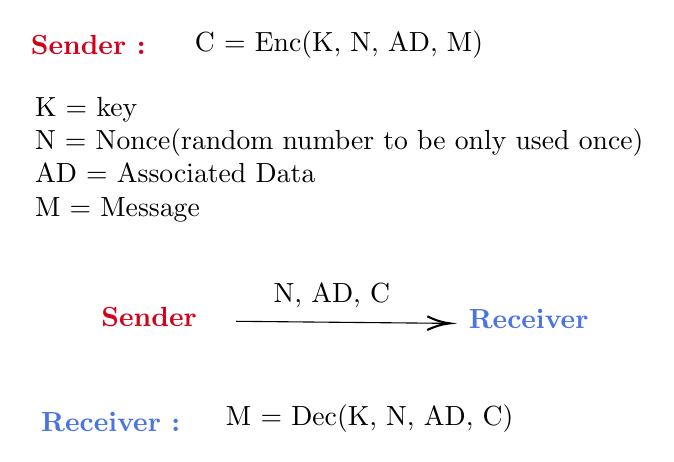
\begin{tikzpicture}[x=0.75pt,y=0.75pt,yscale=-1,xscale=1]
%uncomment if require: \path (0,300); %set diagram left start at 0, and has height of 300

%Straight Lines [id:da22316031770984757] 
\draw    (300.2,187.2) -- (401.2,188.18) ;
\draw [shift={(403.2,188.2)}, rotate = 180.56] [color={rgb, 255:red, 0; green, 0; blue, 0 }  ][line width=0.75]    (10.93,-3.29) .. controls (6.95,-1.4) and (3.31,-0.3) .. (0,0) .. controls (3.31,0.3) and (6.95,1.4) .. (10.93,3.29)   ;

% Text Node
\draw (200,48) node [anchor=north west][inner sep=0.75pt]   [align=left] {\textcolor[rgb]{0.82,0.01,0.11}{\textbf{Sender : }}};
% Text Node
\draw (279,46) node [anchor=north west][inner sep=0.75pt]   [align=left] {C = Enc(K, N, AD, M)};
% Text Node
\draw (202,78) node [anchor=north west][inner sep=0.75pt]   [align=left] {K = key\\N = Nonce(random number to be only used once)\\AD = Associated Data\\M = Message};
% Text Node
\draw (234,179) node [anchor=north west][inner sep=0.75pt]   [align=left] {\textbf{\textcolor[rgb]{0.82,0.01,0.11}{Sender}}};
% Text Node
\draw (411,180) node [anchor=north west][inner sep=0.75pt]   [align=left] {\textbf{\textcolor[rgb]{0.29,0.45,0.89}{Receiver}}};
% Text Node
\draw (317,168) node [anchor=north west][inner sep=0.75pt]   [align=left] {N, AD, C};
% Text Node
\draw (205,230) node [anchor=north west][inner sep=0.75pt]   [align=left] {\textbf{\textcolor[rgb]{0.29,0.45,0.89}{Receiver : }}};
% Text Node
\draw (294,226) node [anchor=north west][inner sep=0.75pt]   [align=left] {M = Dec(K, N, AD, C)};


\end{tikzpicture}
\end{center}

We are sending AD along with the message over the server but AD is not encrypted. If the AD received by the receiver is correct, only then my decryption is valid. So, we can say that AD is authenticating the source of the message. 

\subsection{Details about Signal Protocol}
\begin{itemize}
    \item Generation of shared secret key
    \item Ensuring End-to-End Encryption
    \item Secure Transfer of data from one user to another via Server
    \item Ensuring Forward Secrecy(For example: Even if the secrecy of 10th message is compromised, the previous communication will still be secure). In signal protocol, suppose secrecy of mth message is compromised, still 1 to m-1 messages are secure. Also, messages from m+1 are also secure.
\end{itemize}
This protocol is used in several apps like whatsapp, signal, facebook messenger, skype.\\
It is an open source protocol: \href{https://signal.org/}{https://signal.org/}
\subsection{Main Cryptographic modules of Signal Protocol}
\begin{itemize}
    \item X3DH(Extended Triple Diffie-Hellman)
    \item ECDSA
    \item Double Ratchet
\end{itemize}
X3DH is used to generate the shared keys. ECDSA is used to sign the public keys so that no one else can produce valid public key on behalf of me. Finally Double Ratchet performs the encryption and different keys are generated for every message.\\
\textbf{Note:} Curve X25519 or X448 is used in ECDH and ECDSA.\\
\subsubsection{Registration}
 Alice registers himself to the Server. He has to provide the id to register. Like, for whatsapp, phone number is the id and OTP is used to verify it.
\begin{center}
        

\tikzset{every picture/.style={line width=0.75pt}} %set default line width to 0.75pt        


\begin{tikzpicture}[x=0.75pt,y=0.75pt,yscale=-1,xscale=1]
%uncomment if require: \path (0,300); %set diagram left start at 0, and has height of 300

%Straight Lines [id:da5940913599428925] 
\draw    (169.2,155.6) -- (272.2,155.6) ;
\draw [shift={(274.2,155.6)}, rotate = 180] [color={rgb, 255:red, 0; green, 0; blue, 0 }  ][line width=0.75]    (10.93,-3.29) .. controls (6.95,-1.4) and (3.31,-0.3) .. (0,0) .. controls (3.31,0.3) and (6.95,1.4) .. (10.93,3.29)   ;

% Text Node
\draw (122,146) node [anchor=north west][inner sep=0.75pt]   [align=left] {\textbf{\textcolor[rgb]{0.82,0.01,0.11}{Alice}}};
% Text Node
\draw (277,145) node [anchor=north west][inner sep=0.75pt]   [align=left] {\textbf{\textcolor[rgb]{0.25,0.46,0.02}{Server}}};
% Text Node
\draw (174,127) node [anchor=north west][inner sep=0.75pt]   [align=left] {Registration};


\end{tikzpicture}

\end{center}
During this process, a packet of keys are generated. Let us say that Alice generates the  ${Packet}_A$ which consists of the following:
\begin{itemize}
    \item \textbf{Identity key : ${IK}_A \rightarrow \ (n_{IA}, n_{IA}P)$}\\
    Updated once to the server - Long term
    \item \textbf{Signed prekey : ${SPK}_A \rightarrow \ (n_{SPA}, n_{SPA}P)$}\\
    Updated weekly or once in a month
    \item \textbf{Prekey Signature : Sig(${IK}_A,\ Encode({SPK}_A)$)}\\
    Updated weekly or once in a month\\
     Note: $n_{SPA}P$ is signed using secret key component of ${IK}_A$
    \item \textbf{A set of one-time prekeys : ${{OPK}^1}_A,\ {{OPK}^2}_A,\ {{OPK}^3}_A$}\\
    (Optional) Uploaded when the server requests for it
\end{itemize}
This packet is then uploaded to the server.\\
\vspace{3mm}
Alice then sends ${Packet}_A$ to the Server.\\
\begin{center}
    

\tikzset{every picture/.style={line width=0.75pt}} %set default line width to 0.75pt        


\begin{tikzpicture}[x=0.75pt,y=0.75pt,yscale=-1,xscale=1]
%uncomment if require: \path (0,300); %set diagram left start at 0, and has height of 300

%Straight Lines [id:da5940913599428925] 
\draw    (169.2,155.6) -- (272.2,155.6) ;
\draw [shift={(274.2,155.6)}, rotate = 180] [color={rgb, 255:red, 0; green, 0; blue, 0 }  ][line width=0.75]    (10.93,-3.29) .. controls (6.95,-1.4) and (3.31,-0.3) .. (0,0) .. controls (3.31,0.3) and (6.95,1.4) .. (10.93,3.29)   ;

% Text Node
\draw (122,146) node [anchor=north west][inner sep=0.75pt]   [align=left] {\textbf{\textcolor[rgb]{0.82,0.01,0.11}{Alice}}};
% Text Node
\draw (277,145) node [anchor=north west][inner sep=0.75pt]   [align=left] {\textbf{\textcolor[rgb]{0.25,0.46,0.02}{Server}}};
% Text Node
\draw (192,130) node [anchor=north west][inner sep=0.75pt]   [align=left] {${Packet}_A$};


\end{tikzpicture}
\end{center}
Similarly, Bob will do the same thing.
\begin{center}
    

\tikzset{every picture/.style={line width=0.75pt}} %set default line width to 0.75pt        


\begin{tikzpicture}[x=0.75pt,y=0.75pt,yscale=-1,xscale=1]
%uncomment if require: \path (0,300); %set diagram left start at 0, and has height of 300

%Straight Lines [id:da3983984694334064] 
\draw    (158.2,160.6) -- (267.2,161.58) ;
\draw [shift={(269.2,161.6)}, rotate = 180.52] [color={rgb, 255:red, 0; green, 0; blue, 0 }  ][line width=0.75]    (10.93,-3.29) .. controls (6.95,-1.4) and (3.31,-0.3) .. (0,0) .. controls (3.31,0.3) and (6.95,1.4) .. (10.93,3.29)   ;

% Text Node
\draw (274,147) node [anchor=north west][inner sep=0.75pt]   [align=left] {\textbf{\textcolor[rgb]{0.25,0.46,0.02}{Server}}};
% Text Node
\draw (171,136) node [anchor=north west][inner sep=0.75pt]   [align=left] {Registration};
% Text Node
\draw (113,147) node [anchor=north west][inner sep=0.75pt]   [align=left] {\textbf{\textcolor[rgb]{0.2,0.2,0.55}{Bob}}};


\end{tikzpicture}
\end{center}

Bob generates the ${Packet}_B$ which consists of the following:
\begin{itemize}
    \item \textbf{Identity key : ${IK}_B \rightarrow \ (n_{IB}, n_{IB}P)$}\\
    Updated once to the server - Long term
    \item \textbf{Signed prekey : ${SPK}_B \rightarrow \ (n_{SPB}, n_{SPB}P)$}\\
    Updated weekly or once in a month
    \item \textbf{Prekey Signature : Sig(${IK}_B,\ Encode({SPK}_B)$)}\\
    Updated weekly or once in a month\\
     Note: $n_{SPB}P$ is signed using secret key component of ${IK}_B$
    \item \textbf{A set of one-time prekeys : ${{OPK}^1}_B,\ {{OPK}^2}_B,\ {{OPK}^3}_B$}\\
    (Optional) Uploaded when the server requests for it
\end{itemize}
This packet is then uploaded to the server.\\

\begin{center}
        


\tikzset{every picture/.style={line width=0.75pt}} %set default line width to 0.75pt        


\begin{tikzpicture}[x=0.75pt,y=0.75pt,yscale=-1,xscale=1]
%uncomment if require: \path (0,300); %set diagram left start at 0, and has height of 300

%Straight Lines [id:da3983984694334064] 
\draw    (158.2,160.6) -- (267.2,161.58) ;
\draw [shift={(269.2,161.6)}, rotate = 180.52] [color={rgb, 255:red, 0; green, 0; blue, 0 }  ][line width=0.75]    (10.93,-3.29) .. controls (6.95,-1.4) and (3.31,-0.3) .. (0,0) .. controls (3.31,0.3) and (6.95,1.4) .. (10.93,3.29)   ;

% Text Node
\draw (274,147) node [anchor=north west][inner sep=0.75pt]   [align=left] {\textbf{\textcolor[rgb]{0.25,0.46,0.02}{Server}}};
% Text Node
\draw (171,136) node [anchor=north west][inner sep=0.75pt]   [align=left] {${Packet}_B$};
% Text Node
\draw (113,147) node [anchor=north west][inner sep=0.75pt]   [align=left] {\textbf{\textcolor[rgb]{0.2,0.2,0.55}{Bob}}};


\end{tikzpicture}
\end{center}
Server stores both the packets.
\begin{center}
    

\tikzset{every picture/.style={line width=0.75pt}} %set default line width to 0.75pt        

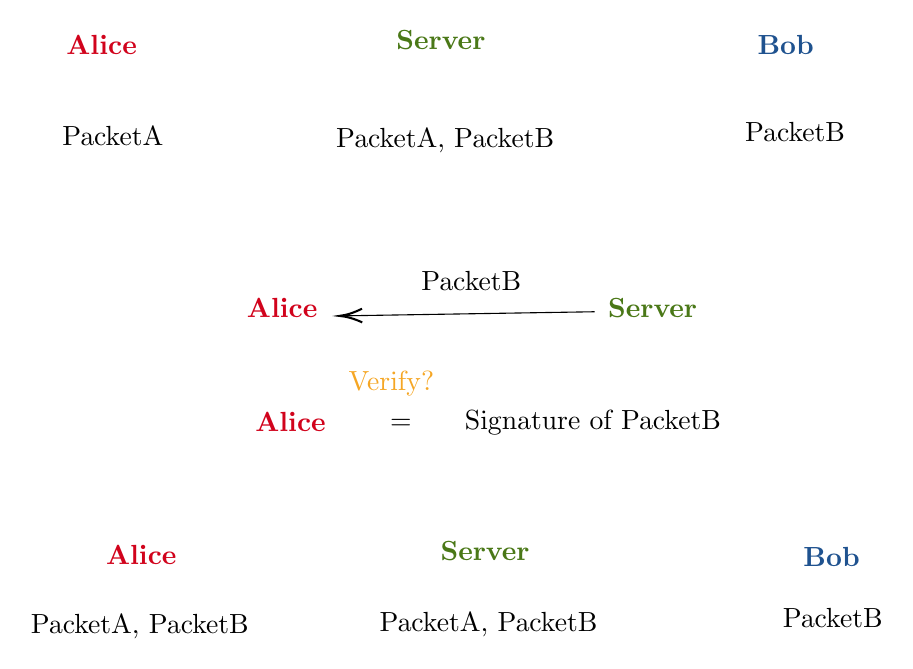
\begin{tikzpicture}[x=0.75pt,y=0.75pt,yscale=-1,xscale=1]
%uncomment if require: \path (0,465); %set diagram left start at 0, and has height of 465

%Straight Lines [id:da22672710839634092] 
\draw    (378.8,196.4) -- (257.8,198.37) ;
\draw [shift={(255.8,198.4)}, rotate = 359.07] [color={rgb, 255:red, 0; green, 0; blue, 0 }  ][line width=0.75]    (10.93,-3.29) .. controls (6.95,-1.4) and (3.31,-0.3) .. (0,0) .. controls (3.31,0.3) and (6.95,1.4) .. (10.93,3.29)   ;

% Text Node
\draw (123,61.8) node [anchor=north west][inner sep=0.75pt]   [align=left] {\textbf{\textcolor[rgb]{0.82,0.01,0.11}{Alice}}};
% Text Node
\draw (282,59.8) node [anchor=north west][inner sep=0.75pt]   [align=left] {\textbf{\textcolor[rgb]{0.29,0.47,0.09}{Server}}};
% Text Node
\draw (456,61.8) node [anchor=north west][inner sep=0.75pt]   [align=left] {\textbf{\textcolor[rgb]{0.12,0.32,0.56}{Bob}}};
% Text Node
\draw (121,105.8) node [anchor=north west][inner sep=0.75pt]   [align=left] {PacketA};
% Text Node
\draw (253,106.8) node [anchor=north west][inner sep=0.75pt]   [align=left] {PacketA, PacketB};
% Text Node
\draw (450,103.8) node [anchor=north west][inner sep=0.75pt]   [align=left] {PacketB};
% Text Node
\draw (210,188.8) node [anchor=north west][inner sep=0.75pt]   [align=left] {\textbf{\textcolor[rgb]{0.82,0.01,0.11}{Alice}}};
% Text Node
\draw (384,188.8) node [anchor=north west][inner sep=0.75pt]   [align=left] {\textbf{\textcolor[rgb]{0.29,0.47,0.09}{Server}}};
% Text Node
\draw (294,175.8) node [anchor=north west][inner sep=0.75pt]   [align=left] {PacketB};
% Text Node
\draw (214,243.8) node [anchor=north west][inner sep=0.75pt]   [align=left] {\textbf{\textcolor[rgb]{0.82,0.01,0.11}{Alice}}};
% Text Node
\draw (279,246.8) node [anchor=north west][inner sep=0.75pt]   [align=left] {=};
% Text Node
\draw (315,242.8) node [anchor=north west][inner sep=0.75pt]   [align=left] {Signature of PacketB};
% Text Node
\draw (259,223.8) node [anchor=north west][inner sep=0.75pt]   [align=left] {\textcolor[rgb]{0.96,0.65,0.14}{Verify?}};
% Text Node
\draw (142.11,307.8) node [anchor=north west][inner sep=0.75pt]   [align=left] {\textbf{\textcolor[rgb]{0.82,0.01,0.11}{Alice}}};
% Text Node
\draw (303.29,305.8) node [anchor=north west][inner sep=0.75pt]   [align=left] {\textbf{\textcolor[rgb]{0.29,0.47,0.09}{Server}}};
% Text Node
\draw (478.11,308.8) node [anchor=north west][inner sep=0.75pt]   [align=left] {\textbf{\textcolor[rgb]{0.12,0.32,0.56}{Bob}}};
% Text Node
\draw (273.87,339.8) node [anchor=north west][inner sep=0.75pt]   [align=left] {PacketA, PacketB};
% Text Node
\draw (468.15,337.8) node [anchor=north west][inner sep=0.75pt]   [align=left] {PacketB};
% Text Node
\draw (105.87,340.8) node [anchor=north west][inner sep=0.75pt]   [align=left] {PacketA, PacketB};


\end{tikzpicture}
\end{center}
Alice verifies the signature using the public key of Bob($n_{IB}P$. Now Alice has all public components of Bob's packet(${IK}_B, \ {SPK}_B$) and her packet(${IK}_A, \ {SPK}_A$). Now she performs the Diffie-Hellman key exchange.
\begin{enumerate}
    \item Alice generates an ephemeral key ${EK}_A$ = $n_{EA}, \ n_{EA}P$
    \item ${DH}_1$ = DH(${IK}_A, \ {SPK}_B$)\\
    DH is performed using $n_{IA}, \ n_{SPB}P$
    \item ${DH}_2$ = DH(${EK}_A, \ {IK}_B$)\\
    DH is performed using $n_{EA}, \ n_{IB}P$
    \item ${DH}_3$ = DH(${EK}_A, \ {SPK}_B$)\\
    DH is performed using $n_{EA}, \ n_{SPB}P$
    \item If key bundle contains one-time prekey,
    \begin{itemize}
        \item ${DH}_4$ = DH(${EK}_A, \ {OPK}_B)$
        \item ${SK}_A$ = KDF(${DH}_1 \ || \ {DH}_2 \ || \  {DH}_3$)
    \end{itemize}
    \item Else ${SK}_A$ = KDF(${DH}_1 \ || \ {DH}_2 \ || \  {DH}_3$)
\end{enumerate}
Here, KDF = SHA-256.
\vspace{3mm}
Now we are done with step 1, that is, X3DH.
Let us move forward.
\begin{enumerate}
    \item Alice computes associated data\\
    AD = Encode(${IK}_A)\ || \ $ Encode(${IK}_B)$\\
    (Only public parts are used here)
    \item Alice encrypts an initial message using AD, ${SK}_A$ and generates the corresponding initial ciphertext.
    \begin{center}
        

\tikzset{every picture/.style={line width=0.75pt}} %set default line width to 0.75pt        

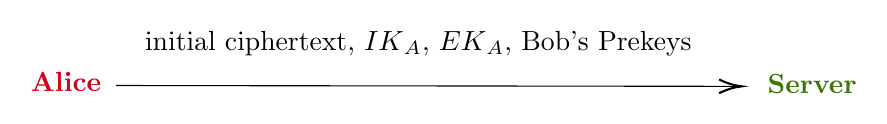
\begin{tikzpicture}[x=0.75pt,y=0.75pt,yscale=-1,xscale=1]
%uncomment if require: \path (0,300); %set diagram left start at 0, and has height of 300

%Straight Lines [id:da5873088927017005] 
\draw    (138.2,140.6) -- (437.8,141) ;
\draw [shift={(439.8,141)}, rotate = 180.08] [color={rgb, 255:red, 0; green, 0; blue, 0 }  ][line width=0.75]    (10.93,-3.29) .. controls (6.95,-1.4) and (3.31,-0.3) .. (0,0) .. controls (3.31,0.3) and (6.95,1.4) .. (10.93,3.29)   ;

% Text Node
\draw (96,133) node [anchor=north west][inner sep=0.75pt]   [align=left] {\textcolor[rgb]{0.82,0.01,0.11}{\textbf{Alice}}};
% Text Node
\draw (451,134) node [anchor=north west][inner sep=0.75pt]   [align=left] {\textbf{\textcolor[rgb]{0.25,0.46,0.02}{Server}}};
% Text Node
\draw (151,113) node [anchor=north west][inner sep=0.75pt]   [align=left] {initial ciphertext, ${IK}_A$, ${EK}_A$, Bob's Prekeys};


\end{tikzpicture}

    \end{center}
    \begin{center}
        

\tikzset{every picture/.style={line width=0.75pt}} %set default line width to 0.75pt        


\begin{tikzpicture}[x=0.75pt,y=0.75pt,yscale=-1,xscale=1]
%uncomment if require: \path (0,300); %set diagram left start at 0, and has height of 300

%Straight Lines [id:da3983984694334064] 
\draw    (158.2,160.6) -- (477.8,159.8) ;
\draw [shift={(479.8,159.8)}, rotate = 179.86] [color={rgb, 255:red, 0; green, 0; blue, 0 }  ][line width=0.75]    (10.93,-3.29) .. controls (6.95,-1.4) and (3.31,-0.3) .. (0,0) .. controls (3.31,0.3) and (6.95,1.4) .. (10.93,3.29)   ;

% Text Node
\draw (487,143) node [anchor=north west][inner sep=0.75pt]   [align=left] 
{\textbf{\textcolor[rgb]{0.2,0.2,0.55}{Bob}}};
% Text Node
\draw (113,147) node [anchor=north west][inner sep=0.75pt]   [align=left] 
{\textbf{\textcolor[rgb]{0.25,0.46,0.02}{Server}}};

% Text Node
\draw (168,139) node [anchor=north west][inner sep=0.75pt]   [align=left] {initial ciphertext, ${IK}_A$, ${EK}_A$, Bob's Prekeys};


\end{tikzpicture}

    \end{center}
    
\end{enumerate}

Now, let us see what happens on Bob's side.
\begin{enumerate}
    \item Bob recovers ${IK}_A$, ${EK}_A$ first.
    \item Bob performs DH(same as Alice) and KDF by using his secret keys.\\
     ${SK}_B$ = KDF(${DH}_1 \ || \ {DH}_2 \ || \  {DH}_3$)
    \item Due to properties of DH and KDF, ${SK}_B$ = ${SK}_A$.
    \item Constructs AD = Encode(${IK}_A)\ || \ $ Encode(${IK}_B)$ (public parts)
    \item Decrypts the initial ciphertext using ${SK}_B)$, AD and recovers the original message.
\end{enumerate}

\begin{center}
    

\tikzset{every picture/.style={line width=0.75pt}} %set default line width to 0.75pt        

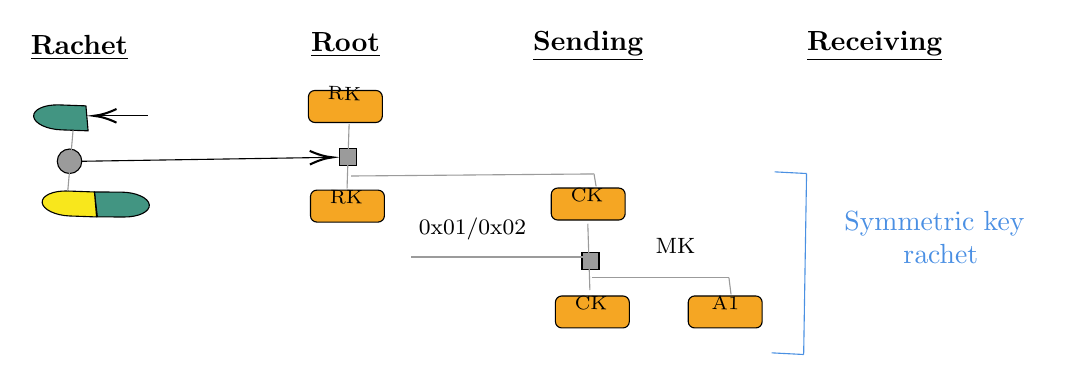
\begin{tikzpicture}[x=0.75pt,y=0.75pt,yscale=-1,xscale=1]
%uncomment if require: \path (0,398); %set diagram left start at 0, and has height of 398

%Flowchart: Delay [id:dp35152848008717874] 
\draw  [fill={rgb, 255:red, 66; green, 149; blue, 130 }  ,fill opacity=1 ] (115.84,193.43) -- (102.99,192.97) .. controls (95.89,192.72) and (89.9,189.82) .. (89.61,186.5) .. controls (89.33,183.17) and (94.85,180.69) .. (101.95,180.94) -- (114.8,181.4) -- cycle ;
%Flowchart: Delay [id:dp16878186037599097] 
\draw  [fill={rgb, 255:red, 66; green, 149; blue, 130 }  ,fill opacity=1 ] (118.9,222.89) -- (131.77,222.96) .. controls (138.87,223) and (144.94,225.71) .. (145.33,229.02) .. controls (145.72,232.34) and (140.27,234.99) .. (133.17,234.95) -- (120.31,234.88) -- cycle ;
%Flowchart: Delay [id:dp959269847195581] 
\draw  [fill={rgb, 255:red, 248; green, 231; blue, 28 }  ,fill opacity=1 ] (119.94,234.92) -- (107.09,234.46) .. controls (99.99,234.21) and (94.01,231.31) .. (93.72,227.98) .. controls (93.43,224.66) and (98.95,222.17) .. (106.05,222.43) -- (118.9,222.89) -- cycle ;
%Rounded Rect [id:dp5324238702681721] 
\draw  [fill={rgb, 255:red, 245; green, 166; blue, 35 }  ,fill opacity=1 ] (405,276.08) .. controls (405,274.38) and (406.38,273) .. (408.08,273) -- (437.52,273) .. controls (439.22,273) and (440.6,274.38) .. (440.6,276.08) -- (440.6,285.32) .. controls (440.6,287.02) and (439.22,288.4) .. (437.52,288.4) -- (408.08,288.4) .. controls (406.38,288.4) and (405,287.02) .. (405,285.32) -- cycle ;
%Rounded Rect [id:dp2780906198381832] 
\draw  [fill={rgb, 255:red, 245; green, 166; blue, 35 }  ,fill opacity=1 ] (222,177.08) .. controls (222,175.38) and (223.38,174) .. (225.08,174) -- (254.52,174) .. controls (256.22,174) and (257.6,175.38) .. (257.6,177.08) -- (257.6,186.32) .. controls (257.6,188.02) and (256.22,189.4) .. (254.52,189.4) -- (225.08,189.4) .. controls (223.38,189.4) and (222,188.02) .. (222,186.32) -- cycle ;
%Rounded Rect [id:dp5179192929824874] 
\draw  [fill={rgb, 255:red, 245; green, 166; blue, 35 }  ,fill opacity=1 ] (223,225.08) .. controls (223,223.38) and (224.38,222) .. (226.08,222) -- (255.52,222) .. controls (257.22,222) and (258.6,223.38) .. (258.6,225.08) -- (258.6,234.32) .. controls (258.6,236.02) and (257.22,237.4) .. (255.52,237.4) -- (226.08,237.4) .. controls (224.38,237.4) and (223,236.02) .. (223,234.32) -- cycle ;
%Rounded Rect [id:dp7787078669609342] 
\draw  [fill={rgb, 255:red, 245; green, 166; blue, 35 }  ,fill opacity=1 ] (339,224.08) .. controls (339,222.38) and (340.38,221) .. (342.08,221) -- (371.52,221) .. controls (373.22,221) and (374.6,222.38) .. (374.6,224.08) -- (374.6,233.32) .. controls (374.6,235.02) and (373.22,236.4) .. (371.52,236.4) -- (342.08,236.4) .. controls (340.38,236.4) and (339,235.02) .. (339,233.32) -- cycle ;
%Rounded Rect [id:dp4090460250497838] 
\draw  [fill={rgb, 255:red, 245; green, 166; blue, 35 }  ,fill opacity=1 ] (341,276.08) .. controls (341,274.38) and (342.38,273) .. (344.08,273) -- (373.52,273) .. controls (375.22,273) and (376.6,274.38) .. (376.6,276.08) -- (376.6,285.32) .. controls (376.6,287.02) and (375.22,288.4) .. (373.52,288.4) -- (344.08,288.4) .. controls (342.38,288.4) and (341,287.02) .. (341,285.32) -- cycle ;
%Shape: Circle [id:dp22137843071657715] 
\draw  [fill={rgb, 255:red, 155; green, 155; blue, 155 }  ,fill opacity=1 ] (101,208.1) .. controls (101,204.84) and (103.64,202.2) .. (106.9,202.2) .. controls (110.16,202.2) and (112.8,204.84) .. (112.8,208.1) .. controls (112.8,211.36) and (110.16,214) .. (106.9,214) .. controls (103.64,214) and (101,211.36) .. (101,208.1) -- cycle ;
%Shape: Square [id:dp30298256876961704] 
\draw  [fill={rgb, 255:red, 155; green, 155; blue, 155 }  ,fill opacity=1 ] (236.8,202) -- (245,202) -- (245,210.2) -- (236.8,210.2) -- cycle ;
%Shape: Square [id:dp8026446713293587] 
\draw  [fill={rgb, 255:red, 155; green, 155; blue, 155 }  ,fill opacity=1 ] (353.8,252) -- (362,252) -- (362,260.2) -- (353.8,260.2) -- cycle ;
%Straight Lines [id:da631551917188083] 
\draw    (112.8,208.1) -- (231.6,206.23) ;
\draw [shift={(233.6,206.2)}, rotate = 179.1] [color={rgb, 255:red, 0; green, 0; blue, 0 }  ][line width=0.75]    (10.93,-3.29) .. controls (6.95,-1.4) and (3.31,-0.3) .. (0,0) .. controls (3.31,0.3) and (6.95,1.4) .. (10.93,3.29)   ;
%Straight Lines [id:da6836683305255884] 
\draw [color={rgb, 255:red, 155; green, 155; blue, 155 }  ,draw opacity=1 ][fill={rgb, 255:red, 155; green, 155; blue, 155 }  ,fill opacity=1 ]   (108.6,193.2) -- (106.05,222.43) ;
%Straight Lines [id:da6222076869270743] 
\draw [color={rgb, 255:red, 155; green, 155; blue, 155 }  ,draw opacity=1 ][fill={rgb, 255:red, 155; green, 155; blue, 155 }  ,fill opacity=1 ]   (241.6,190.2) -- (240.6,221.2) ;
%Straight Lines [id:da15515369902276244] 
\draw [color={rgb, 255:red, 155; green, 155; blue, 155 }  ,draw opacity=1 ][fill={rgb, 255:red, 155; green, 155; blue, 155 }  ,fill opacity=1 ]   (242.6,215.2) -- (359.6,214.2) ;
%Straight Lines [id:da99848657582041] 
\draw [color={rgb, 255:red, 155; green, 155; blue, 155 }  ,draw opacity=1 ][fill={rgb, 255:red, 155; green, 155; blue, 155 }  ,fill opacity=1 ]   (359.6,214.2) -- (360.6,220.2) ;
%Straight Lines [id:da9145338692582143] 
\draw [color={rgb, 255:red, 155; green, 155; blue, 155 }  ,draw opacity=1 ][fill={rgb, 255:red, 155; green, 155; blue, 155 }  ,fill opacity=1 ]   (356.6,238.2) -- (357.6,270.2) ;
%Straight Lines [id:da0496744259888624] 
\draw [color={rgb, 255:red, 155; green, 155; blue, 155 }  ,draw opacity=1 ][fill={rgb, 255:red, 155; green, 155; blue, 155 }  ,fill opacity=1 ]   (358.6,264.2) -- (424.6,264.2) ;
%Straight Lines [id:da24817728829602714] 
\draw [color={rgb, 255:red, 155; green, 155; blue, 155 }  ,draw opacity=1 ][fill={rgb, 255:red, 155; green, 155; blue, 155 }  ,fill opacity=1 ]   (424.6,264.2) -- (425.6,272.2) ;
%Straight Lines [id:da7739020843033195] 
\draw [color={rgb, 255:red, 155; green, 155; blue, 155 }  ,draw opacity=1 ][fill={rgb, 255:red, 155; green, 155; blue, 155 }  ,fill opacity=1 ]   (271.6,254.2) -- (357.1,254.2) ;
%Straight Lines [id:da2684759489667641] 
\draw    (144.6,186.2) -- (120.6,186.2) ;
\draw [shift={(118.6,186.2)}, rotate = 360] [color={rgb, 255:red, 0; green, 0; blue, 0 }  ][line width=0.75]    (10.93,-3.29) .. controls (6.95,-1.4) and (3.31,-0.3) .. (0,0) .. controls (3.31,0.3) and (6.95,1.4) .. (10.93,3.29)   ;
%Straight Lines [id:da9752016308031994] 
\draw [color={rgb, 255:red, 74; green, 144; blue, 226 }  ,draw opacity=1 ]   (462,214) -- (460.6,301.2) ;
%Straight Lines [id:da47232776838299206] 
\draw [color={rgb, 255:red, 74; green, 144; blue, 226 }  ,draw opacity=1 ]   (462,214) -- (446.6,213.2) ;
%Straight Lines [id:da05235231364270754] 
\draw [color={rgb, 255:red, 74; green, 144; blue, 226 }  ,draw opacity=1 ]   (460.6,301.2) -- (445.2,300.4) ;

% Text Node
\draw (87,146) node [anchor=north west][inner sep=0.75pt]   [align=left] {\underline{\textbf{Rachet}}};
% Text Node
\draw (329,144) node [anchor=north west][inner sep=0.75pt]   [align=left] {\textbf{\underline{Sending}}};
% Text Node
\draw (222,145) node [anchor=north west][inner sep=0.75pt]   [align=left] {\underline{\textbf{Root}}};
% Text Node
\draw (461,144) node [anchor=north west][inner sep=0.75pt]   [align=left] {\textbf{\underline{Receiving}}};
% Text Node
\draw (415.22,271.72) node [anchor=north west][inner sep=0.75pt]  [rotate=-1.46] [align=left] {{\scriptsize A1}};
% Text Node
\draw (230.22,170.72) node [anchor=north west][inner sep=0.75pt]  [rotate=-1.46] [align=left] {{\scriptsize RK}};
% Text Node
\draw (231.22,220.72) node [anchor=north west][inner sep=0.75pt]  [rotate=-1.46] [align=left] {{\scriptsize RK}};
% Text Node
\draw (347.22,219.72) node [anchor=north west][inner sep=0.75pt]  [rotate=-1.46] [align=left] {{\scriptsize CK}};
% Text Node
\draw (349.22,271.72) node [anchor=north west][inner sep=0.75pt]  [rotate=-1.46] [align=left] {{\scriptsize CK}};
% Text Node
\draw (274,234) node [anchor=north west][inner sep=0.75pt]   [align=left] {{\footnotesize 0x01/0x02}};
% Text Node
\draw (388,244) node [anchor=north west][inner sep=0.75pt]   [align=left] {{\footnotesize MK}};
% Text Node
\draw (479,231) node [anchor=north west][inner sep=0.75pt]   [align=left] {\begin{minipage}[lt]{69.6pt}\setlength\topsep{0pt}
\textcolor[rgb]{0.29,0.56,0.89}{Symmetric key}
\begin{center}
\textcolor[rgb]{0.29,0.56,0.89}{ rachet}
\end{center}

\end{minipage}};


\end{tikzpicture}

\end{center}

Where RK = root key, CK = chain key. When input is 0x01, new chain key is created. When input is 0x02, A1 is created which is used to encrypt second message. Let us see the chain process.

\begin{center}
    

\tikzset{every picture/.style={line width=0.75pt}} %set default line width to 0.75pt        

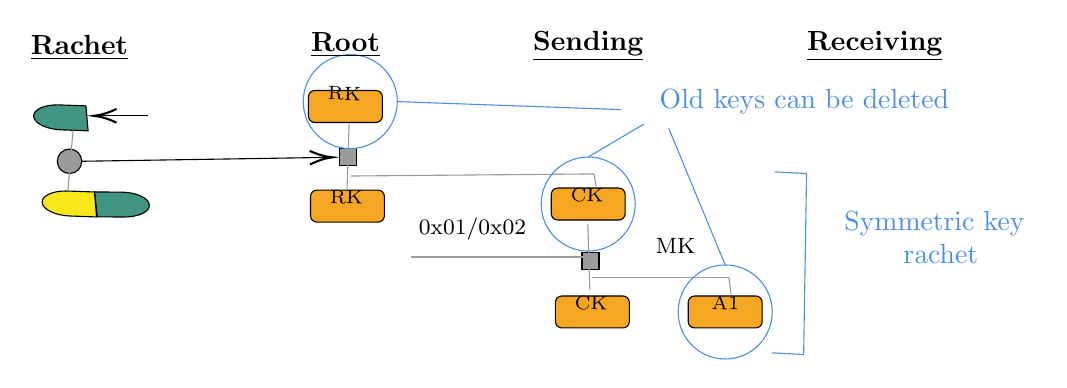
\begin{tikzpicture}[x=0.75pt,y=0.75pt,yscale=-1,xscale=1]
%uncomment if require: \path (0,398); %set diagram left start at 0, and has height of 398

%Flowchart: Delay [id:dp35152848008717874] 
\draw  [fill={rgb, 255:red, 66; green, 149; blue, 130 }  ,fill opacity=1 ] (115.84,193.43) -- (102.99,192.97) .. controls (95.89,192.72) and (89.9,189.82) .. (89.61,186.5) .. controls (89.33,183.17) and (94.85,180.69) .. (101.95,180.94) -- (114.8,181.4) -- cycle ;
%Flowchart: Delay [id:dp16878186037599097] 
\draw  [fill={rgb, 255:red, 66; green, 149; blue, 130 }  ,fill opacity=1 ] (118.9,222.89) -- (131.77,222.96) .. controls (138.87,223) and (144.94,225.71) .. (145.33,229.02) .. controls (145.72,232.34) and (140.27,234.99) .. (133.17,234.95) -- (120.31,234.88) -- cycle ;
%Flowchart: Delay [id:dp959269847195581] 
\draw  [fill={rgb, 255:red, 248; green, 231; blue, 28 }  ,fill opacity=1 ] (119.94,234.92) -- (107.09,234.46) .. controls (99.99,234.21) and (94.01,231.31) .. (93.72,227.98) .. controls (93.43,224.66) and (98.95,222.17) .. (106.05,222.43) -- (118.9,222.89) -- cycle ;
%Rounded Rect [id:dp5324238702681721] 
\draw  [fill={rgb, 255:red, 245; green, 166; blue, 35 }  ,fill opacity=1 ] (405,276.08) .. controls (405,274.38) and (406.38,273) .. (408.08,273) -- (437.52,273) .. controls (439.22,273) and (440.6,274.38) .. (440.6,276.08) -- (440.6,285.32) .. controls (440.6,287.02) and (439.22,288.4) .. (437.52,288.4) -- (408.08,288.4) .. controls (406.38,288.4) and (405,287.02) .. (405,285.32) -- cycle ;
%Rounded Rect [id:dp2780906198381832] 
\draw  [fill={rgb, 255:red, 245; green, 166; blue, 35 }  ,fill opacity=1 ] (222,177.08) .. controls (222,175.38) and (223.38,174) .. (225.08,174) -- (254.52,174) .. controls (256.22,174) and (257.6,175.38) .. (257.6,177.08) -- (257.6,186.32) .. controls (257.6,188.02) and (256.22,189.4) .. (254.52,189.4) -- (225.08,189.4) .. controls (223.38,189.4) and (222,188.02) .. (222,186.32) -- cycle ;
%Rounded Rect [id:dp5179192929824874] 
\draw  [fill={rgb, 255:red, 245; green, 166; blue, 35 }  ,fill opacity=1 ] (223,225.08) .. controls (223,223.38) and (224.38,222) .. (226.08,222) -- (255.52,222) .. controls (257.22,222) and (258.6,223.38) .. (258.6,225.08) -- (258.6,234.32) .. controls (258.6,236.02) and (257.22,237.4) .. (255.52,237.4) -- (226.08,237.4) .. controls (224.38,237.4) and (223,236.02) .. (223,234.32) -- cycle ;
%Rounded Rect [id:dp7787078669609342] 
\draw  [fill={rgb, 255:red, 245; green, 166; blue, 35 }  ,fill opacity=1 ] (339,224.08) .. controls (339,222.38) and (340.38,221) .. (342.08,221) -- (371.52,221) .. controls (373.22,221) and (374.6,222.38) .. (374.6,224.08) -- (374.6,233.32) .. controls (374.6,235.02) and (373.22,236.4) .. (371.52,236.4) -- (342.08,236.4) .. controls (340.38,236.4) and (339,235.02) .. (339,233.32) -- cycle ;
%Rounded Rect [id:dp4090460250497838] 
\draw  [fill={rgb, 255:red, 245; green, 166; blue, 35 }  ,fill opacity=1 ] (341,276.08) .. controls (341,274.38) and (342.38,273) .. (344.08,273) -- (373.52,273) .. controls (375.22,273) and (376.6,274.38) .. (376.6,276.08) -- (376.6,285.32) .. controls (376.6,287.02) and (375.22,288.4) .. (373.52,288.4) -- (344.08,288.4) .. controls (342.38,288.4) and (341,287.02) .. (341,285.32) -- cycle ;
%Shape: Circle [id:dp22137843071657715] 
\draw  [fill={rgb, 255:red, 155; green, 155; blue, 155 }  ,fill opacity=1 ] (101,208.1) .. controls (101,204.84) and (103.64,202.2) .. (106.9,202.2) .. controls (110.16,202.2) and (112.8,204.84) .. (112.8,208.1) .. controls (112.8,211.36) and (110.16,214) .. (106.9,214) .. controls (103.64,214) and (101,211.36) .. (101,208.1) -- cycle ;
%Shape: Square [id:dp30298256876961704] 
\draw  [fill={rgb, 255:red, 155; green, 155; blue, 155 }  ,fill opacity=1 ] (236.8,202) -- (245,202) -- (245,210.2) -- (236.8,210.2) -- cycle ;
%Shape: Square [id:dp8026446713293587] 
\draw  [fill={rgb, 255:red, 155; green, 155; blue, 155 }  ,fill opacity=1 ] (353.8,252) -- (362,252) -- (362,260.2) -- (353.8,260.2) -- cycle ;
%Straight Lines [id:da631551917188083] 
\draw    (112.8,208.1) -- (231.6,206.23) ;
\draw [shift={(233.6,206.2)}, rotate = 179.1] [color={rgb, 255:red, 0; green, 0; blue, 0 }  ][line width=0.75]    (10.93,-3.29) .. controls (6.95,-1.4) and (3.31,-0.3) .. (0,0) .. controls (3.31,0.3) and (6.95,1.4) .. (10.93,3.29)   ;
%Straight Lines [id:da6836683305255884] 
\draw [color={rgb, 255:red, 155; green, 155; blue, 155 }  ,draw opacity=1 ][fill={rgb, 255:red, 155; green, 155; blue, 155 }  ,fill opacity=1 ]   (108.6,193.2) -- (106.05,222.43) ;
%Straight Lines [id:da6222076869270743] 
\draw [color={rgb, 255:red, 155; green, 155; blue, 155 }  ,draw opacity=1 ][fill={rgb, 255:red, 155; green, 155; blue, 155 }  ,fill opacity=1 ]   (241.6,190.2) -- (240.6,221.2) ;
%Straight Lines [id:da15515369902276244] 
\draw [color={rgb, 255:red, 155; green, 155; blue, 155 }  ,draw opacity=1 ][fill={rgb, 255:red, 155; green, 155; blue, 155 }  ,fill opacity=1 ]   (242.6,215.2) -- (359.6,214.2) ;
%Straight Lines [id:da99848657582041] 
\draw [color={rgb, 255:red, 155; green, 155; blue, 155 }  ,draw opacity=1 ][fill={rgb, 255:red, 155; green, 155; blue, 155 }  ,fill opacity=1 ]   (359.6,214.2) -- (360.6,220.2) ;
%Straight Lines [id:da9145338692582143] 
\draw [color={rgb, 255:red, 155; green, 155; blue, 155 }  ,draw opacity=1 ][fill={rgb, 255:red, 155; green, 155; blue, 155 }  ,fill opacity=1 ]   (356.6,238.2) -- (357.6,270.2) ;
%Straight Lines [id:da0496744259888624] 
\draw [color={rgb, 255:red, 155; green, 155; blue, 155 }  ,draw opacity=1 ][fill={rgb, 255:red, 155; green, 155; blue, 155 }  ,fill opacity=1 ]   (358.6,264.2) -- (424.6,264.2) ;
%Straight Lines [id:da24817728829602714] 
\draw [color={rgb, 255:red, 155; green, 155; blue, 155 }  ,draw opacity=1 ][fill={rgb, 255:red, 155; green, 155; blue, 155 }  ,fill opacity=1 ]   (424.6,264.2) -- (425.6,272.2) ;
%Straight Lines [id:da7739020843033195] 
\draw [color={rgb, 255:red, 155; green, 155; blue, 155 }  ,draw opacity=1 ][fill={rgb, 255:red, 155; green, 155; blue, 155 }  ,fill opacity=1 ]   (271.6,254.2) -- (357.1,254.2) ;
%Straight Lines [id:da2684759489667641] 
\draw    (144.6,186.2) -- (120.6,186.2) ;
\draw [shift={(118.6,186.2)}, rotate = 360] [color={rgb, 255:red, 0; green, 0; blue, 0 }  ][line width=0.75]    (10.93,-3.29) .. controls (6.95,-1.4) and (3.31,-0.3) .. (0,0) .. controls (3.31,0.3) and (6.95,1.4) .. (10.93,3.29)   ;
%Straight Lines [id:da9752016308031994] 
\draw [color={rgb, 255:red, 74; green, 144; blue, 226 }  ,draw opacity=1 ]   (462,214) -- (460.6,301.2) ;
%Straight Lines [id:da47232776838299206] 
\draw [color={rgb, 255:red, 74; green, 144; blue, 226 }  ,draw opacity=1 ]   (462,214) -- (446.6,213.2) ;
%Straight Lines [id:da05235231364270754] 
\draw [color={rgb, 255:red, 74; green, 144; blue, 226 }  ,draw opacity=1 ]   (460.6,301.2) -- (445.2,300.4) ;
%Shape: Circle [id:dp7572759422363289] 
\draw  [color={rgb, 255:red, 74; green, 144; blue, 226 }  ,draw opacity=1 ] (219.5,179.35) .. controls (219.5,166.84) and (229.64,156.7) .. (242.15,156.7) .. controls (254.66,156.7) and (264.8,166.84) .. (264.8,179.35) .. controls (264.8,191.86) and (254.66,202) .. (242.15,202) .. controls (229.64,202) and (219.5,191.86) .. (219.5,179.35) -- cycle ;
%Shape: Circle [id:dp16445252309984104] 
\draw  [color={rgb, 255:red, 74; green, 144; blue, 226 }  ,draw opacity=1 ] (334.15,228.7) .. controls (334.15,216.19) and (344.29,206.05) .. (356.8,206.05) .. controls (369.31,206.05) and (379.45,216.19) .. (379.45,228.7) .. controls (379.45,241.21) and (369.31,251.35) .. (356.8,251.35) .. controls (344.29,251.35) and (334.15,241.21) .. (334.15,228.7) -- cycle ;
%Shape: Circle [id:dp811444525661712] 
\draw  [color={rgb, 255:red, 74; green, 144; blue, 226 }  ,draw opacity=1 ] (400.15,280.7) .. controls (400.15,268.19) and (410.29,258.05) .. (422.8,258.05) .. controls (435.31,258.05) and (445.45,268.19) .. (445.45,280.7) .. controls (445.45,293.21) and (435.31,303.35) .. (422.8,303.35) .. controls (410.29,303.35) and (400.15,293.21) .. (400.15,280.7) -- cycle ;
%Straight Lines [id:da8007664732949515] 
\draw [color={rgb, 255:red, 74; green, 144; blue, 226 }  ,draw opacity=1 ]   (264.8,179.35) -- (372.6,183.2) ;
%Straight Lines [id:da35042399495426424] 
\draw [color={rgb, 255:red, 74; green, 144; blue, 226 }  ,draw opacity=1 ]   (356.8,206.05) -- (383.6,190.2) ;
%Straight Lines [id:da19791891775305293] 
\draw [color={rgb, 255:red, 74; green, 144; blue, 226 }  ,draw opacity=1 ]   (422.8,258.05) -- (395.6,192.2) ;

% Text Node
\draw (87,146) node [anchor=north west][inner sep=0.75pt]   [align=left] {\underline{\textbf{Rachet}}};
% Text Node
\draw (329,144) node [anchor=north west][inner sep=0.75pt]   [align=left] {\textbf{\underline{Sending}}};
% Text Node
\draw (222,145) node [anchor=north west][inner sep=0.75pt]   [align=left] {\underline{\textbf{Root}}};
% Text Node
\draw (461,144) node [anchor=north west][inner sep=0.75pt]   [align=left] {\textbf{\underline{Receiving}}};
% Text Node
\draw (415.22,271.72) node [anchor=north west][inner sep=0.75pt]  [rotate=-1.46] [align=left] {{\scriptsize A1}};
% Text Node
\draw (230.22,170.72) node [anchor=north west][inner sep=0.75pt]  [rotate=-1.46] [align=left] {{\scriptsize RK}};
% Text Node
\draw (231.22,220.72) node [anchor=north west][inner sep=0.75pt]  [rotate=-1.46] [align=left] {{\scriptsize RK}};
% Text Node
\draw (347.22,219.72) node [anchor=north west][inner sep=0.75pt]  [rotate=-1.46] [align=left] {{\scriptsize CK}};
% Text Node
\draw (349.22,271.72) node [anchor=north west][inner sep=0.75pt]  [rotate=-1.46] [align=left] {{\scriptsize CK}};
% Text Node
\draw (274,234) node [anchor=north west][inner sep=0.75pt]   [align=left] {{\footnotesize 0x01/0x02}};
% Text Node
\draw (388,244) node [anchor=north west][inner sep=0.75pt]   [align=left] {{\footnotesize MK}};
% Text Node
\draw (479,231) node [anchor=north west][inner sep=0.75pt]   [align=left] {\begin{minipage}[lt]{69.6pt}\setlength\topsep{0pt}
\textcolor[rgb]{0.29,0.56,0.89}{Symmetric key}
\begin{center}
\textcolor[rgb]{0.29,0.56,0.89}{ rachet}
\end{center}

\end{minipage}};
% Text Node
\draw (390,172) node [anchor=north west][inner sep=0.75pt]   [align=left] {\textcolor[rgb]{0.29,0.56,0.89}{Old keys can be deleted}};


\end{tikzpicture}

\end{center}


\begin{figure}[t]
  \includegraphics[width=\linewidth]{signal_chain.png}
\end{figure}

\begin{figure}[h]
  \includegraphics[width=\linewidth]{reply.png}
\end{figure}

\begin{figure}[h]
  \includegraphics[width=\linewidth]{reply2.png}
  \caption{In this figure, we can see the change in sequence of messages because of internet speed.}
\end{figure}

\clearpage % add a page break here

\section{Zero Knowledge Proof using DLP}
Suppose I have certain document and I want to prove that I am the owner of it without sharing the document. 
\begin{figure}[h]
  \includegraphics[width=\linewidth]{DLP.png}
\end{figure}
\begin{center}
    $g^s$ = $g^{ex+r}$ = $g^{ex} \cdot g^r$ = $y^e m$
\end{center}
\section{Recall}
\begin{figure}[htbp]
   \centering
   \includegraphics[width=0.5\textwidth]{ecdh.JPG}
   \caption{Classical Diffie-Hellman on Elliptic Curve}   
\end{figure}
The structure for the AES-128 encryption algorithm is given below.
\begin{figure}[htbp]
   \centering
   \includegraphics[width=0.75\textwidth]{aes.JPG}
   \caption{Structure of AES-128}   
\end{figure}
Although, we will be using the AES-256 but the basic structure remains the same. The AES-256 has only three differences when compared to AES-128. These are mentioned below:
\begin{enumerate}
    \item AES-256 takes a key of length of 256-bits, whereas AES-128 takes 128-bit key as input.
    \item The Number of Rounds in AES-256 are 14 which are 10 for AES-128.
    \item The Key Scheduling Algorithm for AES-256 differs slightly from Key Scheduling Algorithm of AES-128 as more round keys need to be generated in AES-256.
\end{enumerate}
The Key Scheduling Algorithm for both AES-128 and AES-256 are given below.\\
\newline
\begin{figure}[h]
   \centering
   \includegraphics[width=0.75\textwidth]{ks128.JPG}
   \caption{KSA of AES-128}   
\end{figure}
\begin{figure}[h]
   \centering
   \includegraphics[width=0.50\textwidth]{ks256.JPG}
   \caption{KSA of AES-256}   
\end{figure}

\begin{figure}[h]
   \centering
   \includegraphics[width=0.75\textwidth]{encCBC.JPG} 
\end{figure}
\begin{figure}[t]
   \centering
   \includegraphics[width=0.75\textwidth]{decCBC.JPG}
\end{figure}
\end{document}